\chapter{Sistema de Reconhecimento Facial Visage} \label{chap:visage}

\section{Implementação}

\subsection{Sistema de Reconhecimento Facial Base - OpenCV Face Recognizer}
O \textit{OpenCV} é uma biblioteca de código aberto nas áreas de visão por computador e \textit{machine learning}, onde se encontra disponível a implementação de mais de 2500 algoritmos relacionados com as áreas de computação gráfica e visão por computador. Esta biblioteca possui uma comunidade de mais de 47 mil pessoas, já registou mais de 5 milhões de downloads e é utilizada globalmente por empresas como a Google, Yahoo, Microsoft, Intel, IBM, Sony, Honda, Toyota \cite{Team}. 

Ao nível do reconhecimento facial, esta biblioteca disponibiliza um módulo denominado \textit{Face Recognizer}, onde se encontram implementados os algoritmos \textit{Eigenfaces}, \textit{Fisherfaces} e \textit{Local Binary Patterns Histograms}.

Tendo em conta a ampla utilização da biblioteca OpenCV e a sua constante atualização pela comunidade, assim como as facilidades providenciadas pelo módulo de reconhecimento facial, esta foi considerada a biblioteca ideal para utilizar como base de implementação do sistema de reconhecimento facial a criar. De seguida encontram-se brevemente descritas as principais diferenças entre os três algoritmos implementados no módulo \textit{Face Recognizer:}

\subsubsection*{\textit{Eigenfaces}}
O método \textit{Eigenfaces} foi introduzido por Turk e Pentland em 1991 \cite{Turk1991}, e tira partido da Análise dos Componentes Principais (ACP) para efetuar o reconhecimento facial automático.

A análise de componentes principais tem como objetivo determinar as relações existentes entre diferentes conjuntos de dados, nomeadamente ao nível das suas diferenças e semelhanças, tirando partido da redundância existente para criar uma representação reduzida dos dados sem que a perda de informação ocorrida seja significativa. As imagens faciais possuem uma grande redundância natural, o algoritmo \textit{Eigenfaces}, através da análise dos componentes principais dessas imagens, efetua uma projeção das imagens faciais num sub-espaço onde se evidenciam apenas as variações entre as diversas caras conhecidas pelo sistema.

A redução do espaço de representação revela-se fulcral no problema de reconhecimento facial em imagens, devido à grande dimensionalidade exigida para a representação de uma face. Considerando, por exemplo, uma dada imagem de $n$ x $m$ \textit{pixels} de tons cinzentos, essa imagem poderia ser traduzida por um espaço vetorial de $m = $ $n$ x $m$ \textit{pixels}, assim sendo, uma imagem de apenas $256x256$ \textit{pixels} necessitaria de um total de $65536$ \textit{pixels} para ser representada.

O processo de reconhecimento facial com recurso ao algoritmo \textit{Eigenfaces} consiste nos seguintes passos:
\begin{enumerate}
\item Aquisição de um conjunto de dados iniciais (conjunto de treino);
\item Projeção dos dados obtidos num sub-espaço de faces através da ACP;
\item Aquisição de uma imagem a reconhecer;
\item Projeção da face a reconhecer no sub-espaço do conjunto de treino, calculando as distâncias obtidas para cada face conhecida pelo sistema;
\item Determinar qual a face do conjunto de treino com menor distância à face a reconhecer;
\item Caso a distância para a face obtida seja menor do que um limite operacional estabelecido, a imagem é reconhecida como sendo essa pessoa, caso contrário, a face é identificada como sendo uma pessoa desconhecida pelo sistema.
\end{enumerate}

Este método efetua assim uma abordagem holística ao problema de reconhecimento facial em imagens, uma vez que tem em consideração a representação facial como um todo, não fazendo a distinção entre pontos específicos da face como olhos, orelhas ou nariz para efetuar o reconhecimento facial. Uma vantagem deste tipo de representação é a reduzida sensibilidade ao ruído presente nas imagens \cite{Zhao2003}.

\subsubsection*{\textit{Fisherfaces}}
A análise dos componentes principais visa determinar o sub-espaço onde se verifica uma maior variação entre um conjunto de imagens. No entanto, a variação na representação facial de uma pessoa encontra-se muitas vezes relacionada com mudanças de expressões faciais ou iluminação dos indivíduos, pelo que, o sub-espaço criado pelo algoritmo \textit{Eigenfaces} não traduz muitas vezes apenas as diferenças de identidade entre os diversos indivíduos, mas também as diferenças verificadas entre as várias representações de um indivíduo devido à variação nas condições de captura das imagens. O algoritmo \textit{Fisherfaces} \cite{Belhumeur1997, Etemad1997, Zhao1998}, tenta resolver este problema, através da aplicação de um passo de Análise Linear Discriminante (ALD) \textit{(Linear Discriminant analysis)} após a análise dos componentes principais, de forma a determinar mais corretamente as variações intra-classe existentes no conjunto de imagens a avaliar.

A ALD, inicialmente introduzida por Fisher em 1936 \cite{FISHER1936}, tenta maximizar as diferenças existentes entre diferentes indivíduos(inter-classe) e minimizar as variações entre imagens da mesma pessoa(intra-classe) de modo a obter uma representação mais robusta em termos de variação ao nível da iluminação. Após a aplicação dos passos de ACP e ALD, o processo de reconhecimento do método \textit{Fisherfaces} é semelhante ao efetuado pelo método \textit{Eigenfaces}, sendo também efetuada uma abordagem holística ao reconhecimento facial.


\subsubsection*	{\textit{Local Binary Patterns Histograms (LBPH)}}
Ao contrário dos algoritmos descritos anteriormente, o LBPH efetua uma abordagem local ao problema de reconhecimento facial, efetuando uma extração das características locais de uma imagem. Este tipo de abordagem possuí a vantagem de possuir uma baixa dimensionalidade implícita, pelo que não existe a necessidade de efetuar a projeção das imagens num sub-espaço.

A ideia base das \textit{Local Binary Patterns (LBP)}, consiste em resumir a estrutura local de imagem através de uma comparação de um pixel com os seus vizinhos. Dado um pixel central é analisada a diferença entre esse pixel e cada um dos seus vizinhos. Se a intensidade do pixel for maior ou igual do que a do seu vizinho é atribuído o valor 1, caso contrário é atribuído o valor 0. Cada pixel pode então ser traduzido por um número binário do género $11001111$. Dados $8$ pixeis é então possível efetuar $2^8$ combinações, cada uma designada de LBP.

Ahonen \textit{et al.} \cite{ahonen2004face}, propuseram o uso de LBP para o reconhecimento facial em imagens. A sua abordagem consiste na divisão da face em pequenas regiões das quais são derivadas LBP e concatenas numa representação única designada de LBPH, a qual representa uma imagem facial. O reconhecimento é depois efetuado através do determinação do vizinho mais próximo no espaço de faces computado.

\subsection{Filtros de Abstração - Filtro Kuwahara Anisotrópico}
\begin{figure}[ht]
  \begin{center}
    \leavevmode
    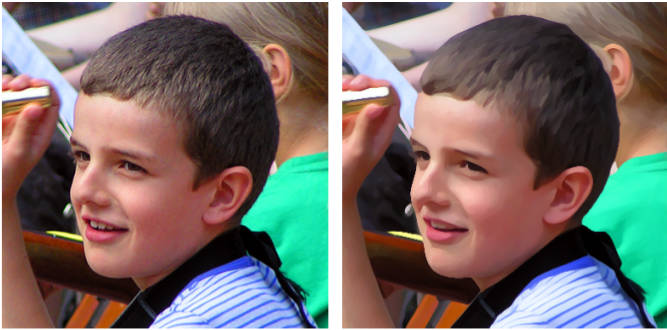
\includegraphics[width=0.7\textwidth]{filterskid}
    \caption{Comparação entre imagem não abstraída (esquerda) e imagem abstraída (direita) \cite{Kyprianidis2009}.}	
    \label{fig:filterskid}
  \end{center}
\end{figure}

Ao nível dos filtros de abstração o estudo será efetuado utilizado o filtro Kuwahara Anisotrópico (FKA).

Este filtro consiste numa generalização do filtro Kuwahara (ver \ref{subsec:kuwahara}) que remove alguns artefactos originados na aplicação do filtro original através da adaptação da forma, escala e orientação do filtro à estrutura local das características da imagem \cite{Kyprianidis2009}. Desta forma é produzido um efeito de abstração tipo pintura, onde é removida informação não essencial em zonas de elevado contraste, enquanto são preservados os limites representados nas zonas de menor contraste, tal como demonstrado na figura \ref{fig:filterskid}. As imagens ficam assim com a clareza de uma ilustração, mas preservam a informação direcional tal como nas pinturas a óleo clássicas. Por outro lado, este filtro tira partido da placa gráfica para a realização da abstração das imagens, tornando-se assim particularmente indicado para o processamento de um elevado número de fotografias.

O filtro em questão foi também utilizado anteriormente, e com resultados positivos, em abstração de imagens para a recuperação de informação multimédia. 

Tendo em conta os fatores apresentados consideramos que este filtro é o mais adequado para a utilização no âmbito deste projeto.
	
\section{Arquitectura}

	diagrama com a pipeline
	
	descrição dos módulos
	
\section{Detalhes Implementação}
...

\begin{figure}[ht]
  \begin{center}
    \leavevmode
    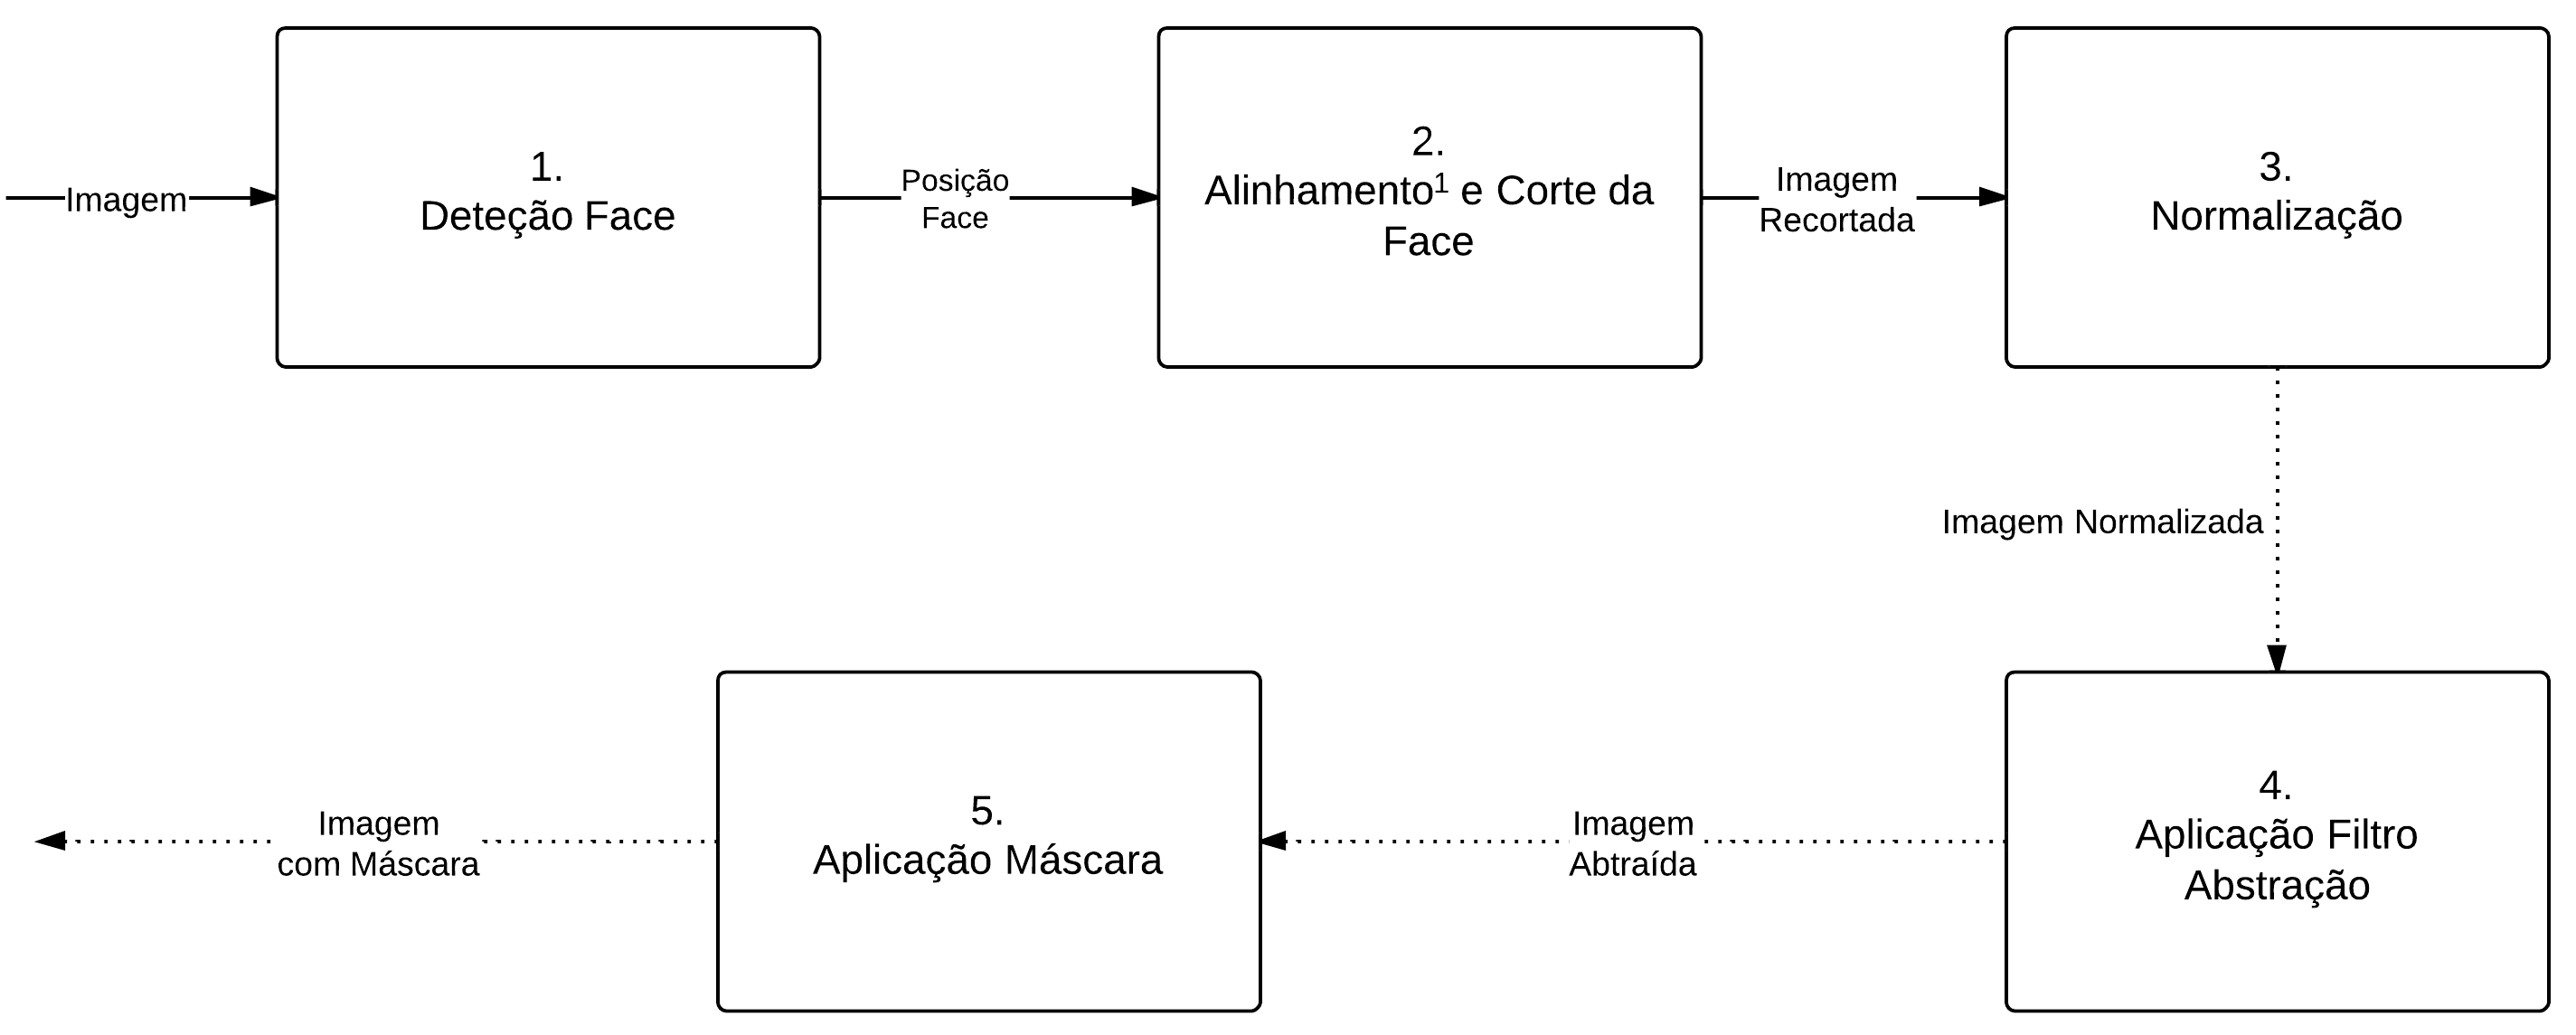
\includegraphics[width=0.7\textwidth]{PreProcessamentoVisage}
    \caption{Cadeia de pré-processamento a que as imagens podem ser sujeitas.}
    \label{fig:preprocessamento}
  \end{center}
\end{figure}

O passo 1 é responsável pela deteção da localização da face na imagem e efetuar a respectiva segmentação da mesma, de acordo com descrito em \ref{chap:detector}. Após a obtenção da face extraída da imagem é então possível proceder à sua normalização em termos de contraste. Para isso foram analisadas três possibilidades: \textit{contrast streching}, \textit{histogram equalization} e ainda \textit{CLAHE}. Posteriormente a imagem po....


\section{Funcionalidades}

	API?
